\title{Computer Vision Assignment-2}
\author{Abhinav Gupta (NetID-ag5799)}
\date{\today}

\documentclass[11pt]{article}

\usepackage{amsfonts,amsmath}
\usepackage{latexsym}
\usepackage{fullpage}
\usepackage{graphicx}
\usepackage{caption}
\usepackage{subcaption}
\usepackage{float}

\begin{document}
\maketitle

2. The images for the MNIST and CIFAR training data are as follows:
\begin{figure}[H]
\begin{subfigure}{.5\textwidth}
\centering
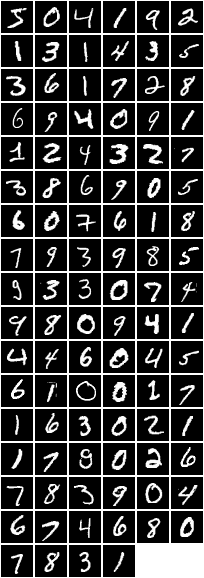
\includegraphics[scale=0.5]{assign2/torch/mnist100.png}
\caption{MNIST-100 \label{fig1}}
\end{subfigure}
\begin{subfigure}{.5\textwidth}
\centering
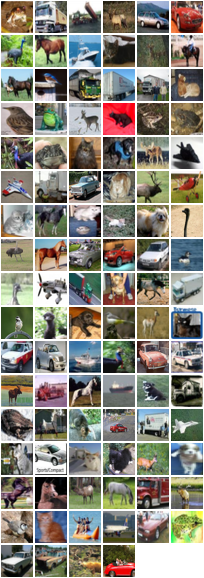
\includegraphics[scale=0.5]{assign2/torch/cifar100.png}
\caption{CIFAR-100 \label{fig2}}
\end{subfigure}
\end{figure}

3.(a) The output after training, validating and testing on 1000 examples.
\begin{figure}[H]
\centering
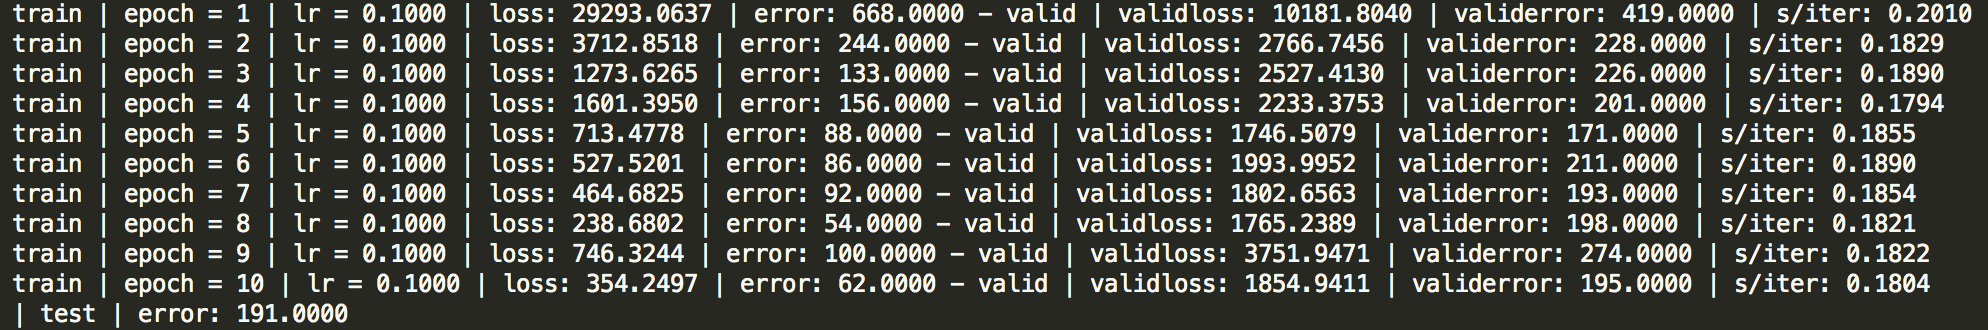
\includegraphics[scale=0.5]{assign2/torch/output1000.png}
\caption{ \label{fig5}}
\end{figure}
(b) The output after training on 50 examples and using the full validation and test set.
\begin{figure}[H]
\centering
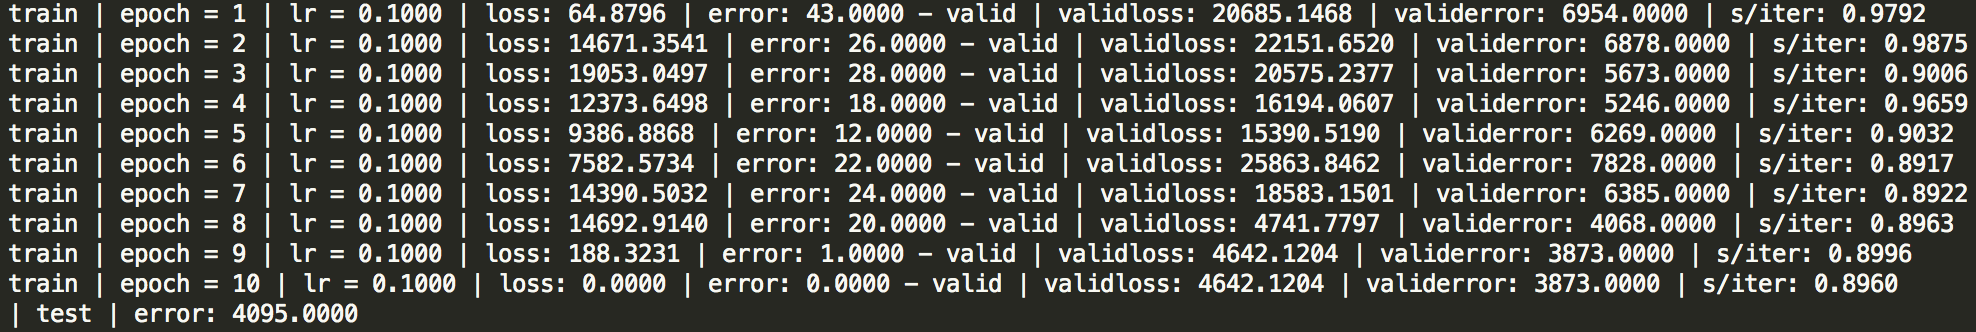
\includegraphics[scale=0.5]{assign2/torch/output50.png}
\caption{ \label{fig6}}
\end{figure}
Visualization of the network weights for both models:
\begin{figure}[H]
\begin{subfigure}{.5\textwidth}
\centering
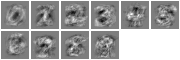
\includegraphics{assign2/torch/weight_1000.png}
\caption{Weights for 1000 examples\label{fig3}}
\end{subfigure}
\begin{subfigure}{.5\textwidth}
\centering
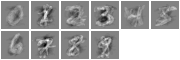
\includegraphics{assign2/torch/weight_50.png}
\caption{Weights for 50 examples\label{fig4}}
\end{subfigure}
\end{figure}

4.(a)
\begin{figure}[H]
\centering
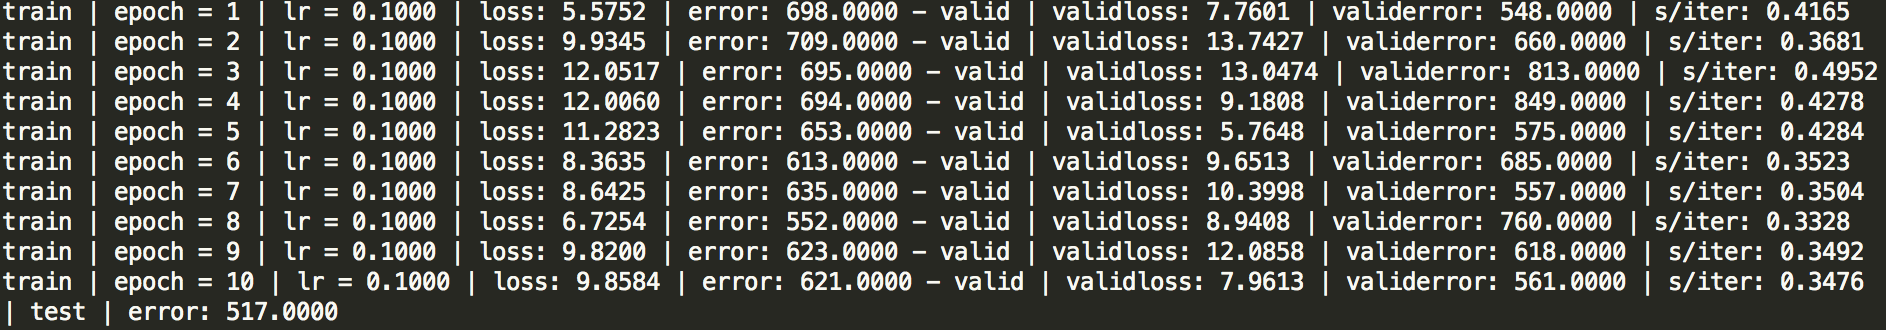
\includegraphics[scale=0.5]{assign2/torch/outputLRpoint1.png}
\caption{ \label{fig5}}
\end{figure}

(b)
\begin{figure}[H]
\centering
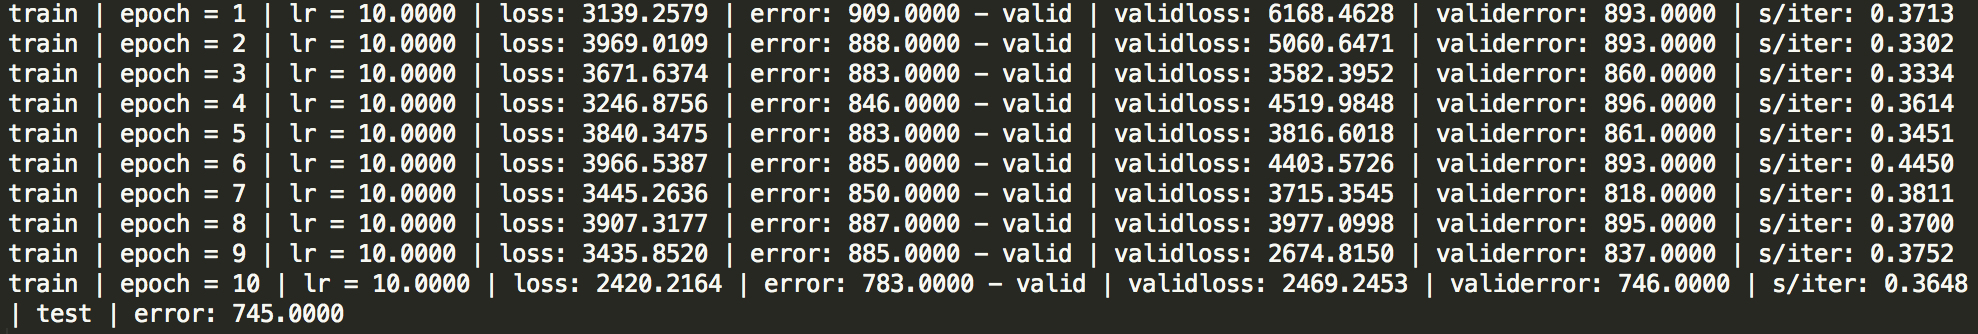
\includegraphics[scale=0.5]{assign2/torch/outputLR10.png}
\caption{ \label{fig5}}
\end{figure}
Due to high learning rate, the model keeps on jumping back and forth in the curve. The \\
5.(a)
\begin{figure}[H]
\centering
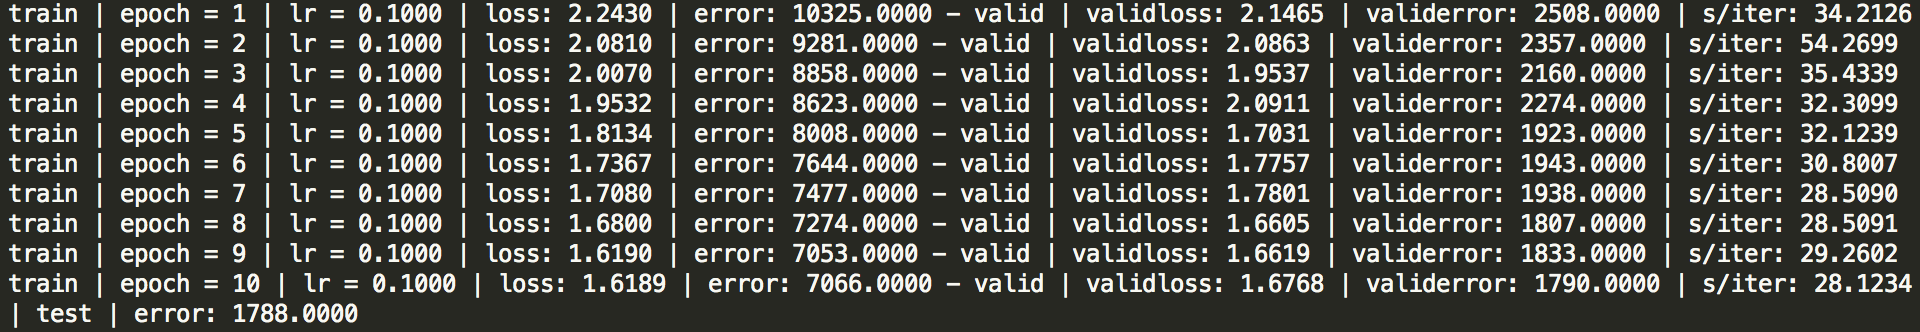
\includegraphics[scale=0.5]{assign2/torch/outputCNN.png}
\caption{ \label{fig5}}
\end{figure}
 
\begin{figure}[H]
\centering
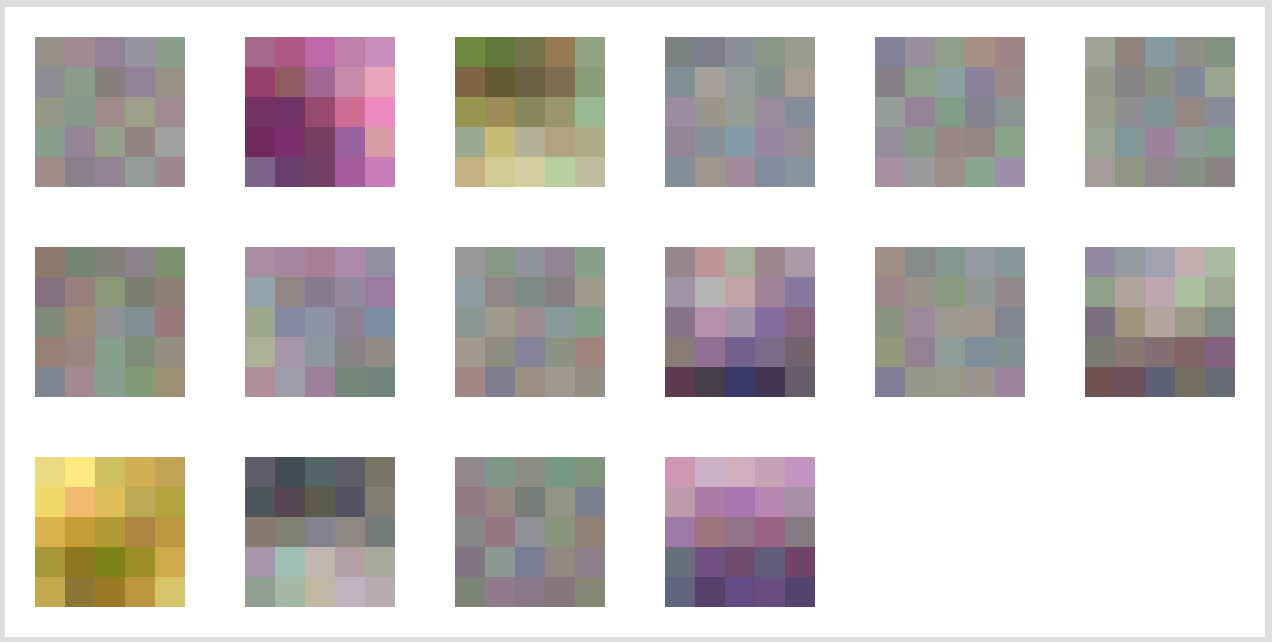
\includegraphics[scale=0.5]{assign2/torch/weightCNN.png}
\caption{Image of first layer filters \label{fig5}}
\end{figure}

(b) The parameters of the model are as follows: \\
1. Convolutional Layer (16((5x5x3)+1)) for 16 filters of 5x5x3 and 1 bias for each  = 1216\\
2. NonLinearity Layer-Tanh (No parameters) = 0\\
3. MaxPooling Layer (No parameters) = 0\\
4. Convolutional Layer (128((5x5x16)+1)) for 128 filters of 5x5x16 and 1 bias for each  = 51328\\
5. NonLinearity Layer-Tanh (No parameters) = 0 \\
6. MaxPooling Layer (No parameters) = 0\\
7. Linear Layer (64((128x5x5)+1)) for 3200 units connected to 64 units each output having 1 bias = 204864\\
8. Linear Layer (10(64+1)) for 64 units connected to 10 units each output having 1 bias = 650 \\
So, total number of parameters = 258058
\end{document}	
